% -*- latex -*-
%%%%%%%%%%%%%%%%%%%%%%%%%%%%%%%%%%%%%%%%%%%%%%%%%%%%%%%%%%%%%%%%
%%%%%%%%%%%%%%%%%%%%%%%%%%%%%%%%%%%%%%%%%%%%%%%%%%%%%%%%%%%%%%%%
%%%%
%%%% This text file is part of the source of 
%%%% `Parallel Programming in MPI and OpenMP'
%%%% by Victor Eijkhout, copyright 2012-2023
%%%%
%%%% mpi-blocksend.tex : blocking sends
%%%%
%%%%%%%%%%%%%%%%%%%%%%%%%%%%%%%%%%%%%%%%%%%%%%%%%%%%%%%%%%%%%%%%
%%%%%%%%%%%%%%%%%%%%%%%%%%%%%%%%%%%%%%%%%%%%%%%%%%%%%%%%%%%%%%%%

\Level 0 {Blocking point-to-point operations}

Suppose you have an array of numbers $x_i\colon i=0,\ldots,N$
and you want to compute
\[ y_i=(x_{i-1}+x_i+x_{i+1})/3\colon i=1,\ldots,N-1. \]
As seen in figure~\ref{fig:mpi-array}, we give each processor
a contiguous subset of the~$x_i$s and $y_i$s.
Let's define $i_p$ as the first index of~$y$ that is
computed by processor~$p$. (What is the last index computed by processor~$p$?
How many indices are computed on that processor?)

We often talk about the \indexterm{owner computes}
model of parallel computing: each processor `owns' certain data items,
and it computes their value. The values used for this computation
need of course not be local, and this is where the need for
communication arises.

\begin{comment}
  %
  \begin{figure}[t]
    \includegraphics[scale=.3]{threepoint-scheme}
    \caption{Three point averaging}
    \label{fig:3pt}
  \end{figure}
  %
\end{comment}

\begin{figure}[t]
  \includegraphics[scale=.12]{threepoint-interior}
  \caption{Three point averaging in parallel, case of interior points}
  \label{fig:3pt-interior}
\end{figure}
%
Let's investigate how processor~$p$ goes about computing~$y_i$ for
the $i$-values it owns. Let's assume that process~$p$ also stores
the values $x_i$ for these same indices.
Now, for many values~$i$ it can evalute the computation
\[ y_{i} = (x_{i-1}+x_{i}+x_{i+1})/3 \]
locally (figure~\ref{fig:3pt-interior}).

However, there is a problem with computing~$y$
in the first index $i_p$ on processor~$p$:
\[ y_{i_p} = (x_{i_p-1}+x_{i_p}+x_{i_p+1})/3 \]
The point to the left, $x_{i_p-1}$,
is not stored on process~$p$
(it is stored on~$p-\nobreak1$),
so it is not immediately available for use by process~$p$.
%
\begin{figure}[t]
  \includegraphics[scale=.12]{threepoint-msg}
  \caption{Three point averaging in parallel, case of edge points}
  \label{fig:3pt-msg}
\end{figure}
%
(figure~\ref{fig:3pt-msg}).
There is a similar story with the last index that $p$ tries to compute:
that involves a value that is only present on~$p+1$.

You see that there is a need for processor-to-processor, or
technically \indexterm{point-to-point}, information exchange.
MPI realizes this through matched send and receive calls:
\begin{itemize}
\item One process does a send to a specific other process;
\item the other process does a specific receive from that source.
\end{itemize}

We will now discuss the send and receive routines in detail.

\Level 1 {Example: ping-pong}
\label{sec:mpi-send-recv}

A simple scenario for information exchange between just two processes
is the \indexterm{ping-pong}: process~A sends data to process~B, which
sends data back to~A.
This is not an operation that is particularly relevant to applications,
although it is often used as a benchmark.
Here we discuss it for to explain basic ideas.

This means that process~A executes the code
\begin{lstlisting}
MPI_Send( /* to: */ B ..... );
MPI_Recv( /* from: */ B ... );
\end{lstlisting}
while process~B executes
\begin{lstlisting}
MPI_Recv( /* from: */ A ... );
MPI_Send( /* to: */ A ..... );
\end{lstlisting}
Since we are programming in SPMD mode, this means our program looks like:
\begin{lstlisting}
if ( /* I am process A */ ) {
  MPI_Send( /* to: */ B ..... );
  MPI_Recv( /* from: */ B ... );
} else if ( /* I am process B */ ) {
  MPI_Recv( /* from: */ A ... );
  MPI_Send( /* to: */ A ..... );
}
\end{lstlisting}

\begin{remark}
  The structure of the send and receive calls shows the symmetric nature of MPI: every
  target process is reached with the same send call, no matter whether it's
  running on the same multicore chip as the sender, or on a
  computational node halfway across the machine room, taking
  several network hops to reach. Of course, any
  self-respecting MPI implementation optimizes for the case where sender
  and receiver have access to the same shared memory.
  This means that a send/recv pair is realized as
  a copy operation from the sender buffer to the
  receiver buffer, rather than a network transfer.
\end{remark}

\Level 1 {Send call}

The blocking send command is
%
\indexmpiref{MPI_Send}.
%
Example:
\cverbatimsnippet[examples/mpi/c/sendandrecv.c]{sendexample}

The send call has the following elements.

\heading{Buffer}
The \indextermbus{send}{buffer} is described by a trio of buffer/count/datatype.
See section~\ref{sec:mpi-buffers} for discussion.

\heading{Target}
The  \indextermbusdef{messsage}{target} is an
explicit process rank to send to.  This rank is a number from zero up
to the result of \indexmpishow{MPI_Comm_size}.
It is allowed for a process to send to itself, but
this may lead to a runtime \indexterm{deadlock};
see section~\ref{sec:blocking} for discussion.
The value \indexmpishow{MPI_PROC_NULL} is allowed:
using that as a target causes no message to be sent
or received.

\heading{Tag}
Next, a message can have a
\emph{tag}\index{tag|see{message, tag}}\index{message!tag}.
Many applications have each sender send only one message at a time
to a given receiver.
For the case where there are
multiple simultaneous messages between the same sender~/ receiver pair,
the tag can be used to disambiguate between
the messages.

Often, a tag value of zero is safe to use.
Indeed, \ac{OO} interfaces to MPI typically have  the tag
as an optional parameter with value zero.
If you do
use tag values, you can use the key \indexmpishow{MPI_TAG_UB} to query
what the maximum value is that can be used; see
section~\ref{sec:mpi_attr}.

\heading{Communicator}
Finally, in common with the vast majority of MPI calls,
there is a communicator argument that provides a context for the send transaction.
In order to match a send and receive operation,
they need to be in the same communicator.

\begin{mplnote}{Buffer type safety}
  \begin{itemize}
  \item Data type is templated: derived by the compiler.
  \item Count $>1$ is declared in the datatype.
  \end{itemize}
\end{mplnote}

\begin{mplnote}{Blocking send and receive}
  \ac{MPL} uses a default value for the tag, and it can deduce the type
  of the buffer. Sending a scalar becomes:
  %
  \cxxverbatimsnippet[examples/mpi/mpl/sendscalar.cxx]{mplsendscalar}
  %
  (See also note~\ref{mpl:buf-scalar}.)
\end{mplnote}

\begin{mplnote}{Sending arrays}
  \ac{MPL} can send \indextermsub{static}{array}s
  without further layout specification:
  %
  \cxxverbatimsnippet[examples/mpi/mpl/sendarray.cxx]{mplsendarray}

  Sending vectors uses a general mechanism:
  %
  \cxxverbatimsnippet[examples/mpi/mpl/sendbuffer.cxx]{mplsendbuffer}
  
  (See also note~\ref{mpl:vec-buf}.)
\end{mplnote}

\begin{comment}
  \begin{mplnote}{Iterator buffers}
    It is possible to to send containers by iterators
    %
    \cxxverbatimsnippet[examples/mpi/mpl/sendrange.cxx]{mplsendrange}
  \end{mplnote}
\end{comment}

\begin{mplnote}{Iterator layout}
  Noncontiguous iteratable objects can be send with a
  \indexmpldef{iterator_layout}:
  %
\begin{lstlisting}
std::list<int> v(20, 0);
mpl::iterator_layout<int> l(v.begin(), v.end());
comm_world.recv(&(*v.begin()), l, 0);  
\end{lstlisting}
(See also note~\ref{mpl:buf-itr}.)
\end{mplnote}

\Level 1 {Receive call}

The basic blocking receive command is
\indexmpiref{MPI_Recv}.

An example:
%
\cverbatimsnippet[examples/mpi/c/sendandrecv.c]{recvexample}

This is similar in structure to the send call, with some exceptions.

\heading{Buffer}
The \indextermsub{receive}{buffer} has the same buffer/count/data parameters as the send
call.
However, 
the \lstinline{count} argument here indicates the size of the buffer,
rather than the actual length of a message.
This sets an upper bound on the length of the incoming message.
\begin{itemize}
\item For receiving messages with unknown length, use \indexmpishow{MPI_Probe};
  section~\ref{sec:mpi-probe}.
\item A message longer than the buffer size will give an overflow error,
  either returning an error, or ending your program; see section~\ref{sec:mpi-error}.
\end{itemize}
The length of the received message can be determined 
from the status object; see section~\ref{sec:mpi-status} for more detail.

\heading{Source}
Mirroring the target argument of the \indexmpishow{MPI_Send} call,
\indexmpishow{MPI_Recv} has a \indextermbusdef{message}{source}
argument.
This can be either a specific rank, or it can be the
\indexmpidef{MPI_ANY_SOURCE} wildcard. In the latter case, the actual
source can be determined after the message has been received;
see section~\ref{sec:mpi-status}.
A~source value of \indexmpishow{MPI_PROC_NULL} is also allowed,
which makes the receive succeed immediately with no data received.

\begin{mplnote}{Any source}
  The constant \lstinline+mpl::+\indexmplshow{any_source}
  equals \indexmpishow{MPI_ANY_SOURCE} (by \lstinline+constexpr+).
\end{mplnote}

\heading{Tag}
Similar to the messsage source, the message tag of a receive call can
be a specific value or a wildcard, in this case
\indexmpidef{MPI_ANY_TAG}.

\begin{pythonnote}{Message tags}
  Python calls sensible use a default \lstinline{tag=0},
  but you can specify your own tag value.
  On the receive call, the tag wildcard is \indexmpishow{MPI.ANY_TAG}.
\end{pythonnote}

\heading{Communicator}
The communicator argument almost goes without remarking.

\heading{Status}
The \indexmpishow{MPI_Recv} command has one parameter that
the send call lacks: the \indexmpishow{MPI_Status} object,
describing the \indextermbus{message}{status}.
This gives information about the message received,
for instance if you used wildcards for source or tag.
See section~\ref{sec:mpi-status}
for more about the status object.

\begin{remark}
  If you're not interested in the status,
  as is the case in many examples in this book,
  you can specify the constant \indexmpidef{MPI_STATUS_IGNORE}.
  Note that the signature of \indexmpishow{MPI_Recv} lists the status parameter
  as `output'; this `direction' of the parameter of course only applies
  if you do not specify this constant.
\end{remark}

\begin{exercise}
  \label{ex:pingpong}
  Implement the ping-pong program. Add a timer using \indexmpishow{MPI_Wtime}.
  For the \n{status} argument of the receive call, use
  \indexmpishow{MPI_STATUS_IGNORE}.

  \begin{itemize}
  \item Run multiple ping-pongs (say a thousand) and put the timer
    around the loop. The first run may take longer; try to discard it.
  \item Run your code with the two communicating processes first on
    the same node, then on different nodes. Do you see a difference?
  \item Then modify the program
    to use longer messages. How does the timing increase with message size?
  \end{itemize}
  For bonus points, can you do a regression to determine~$\alpha,\beta$?
  \skeleton{pingpong}
\end{exercise}

\begin{exercise}
  \label{ex:hbwpingpong}
  Take your pingpong program and modify it 
  to let half the processors
  be source and the other half the targets. Does the pingpong time increase?
  Does the observed behavior depend on how you choose the two sets?
\end{exercise}

\Level 1 {Problems with blocking communication}
\label{sec:blocking}
\index{communication!blocking|(textbf}

You may be tempted to think that the send call puts the data somewhere
in the network, and the sending code can progress after this call,
as in figure~\ref{fig:send-ideal}, left.
%
\begin{figure}[ht]
\leavevmode
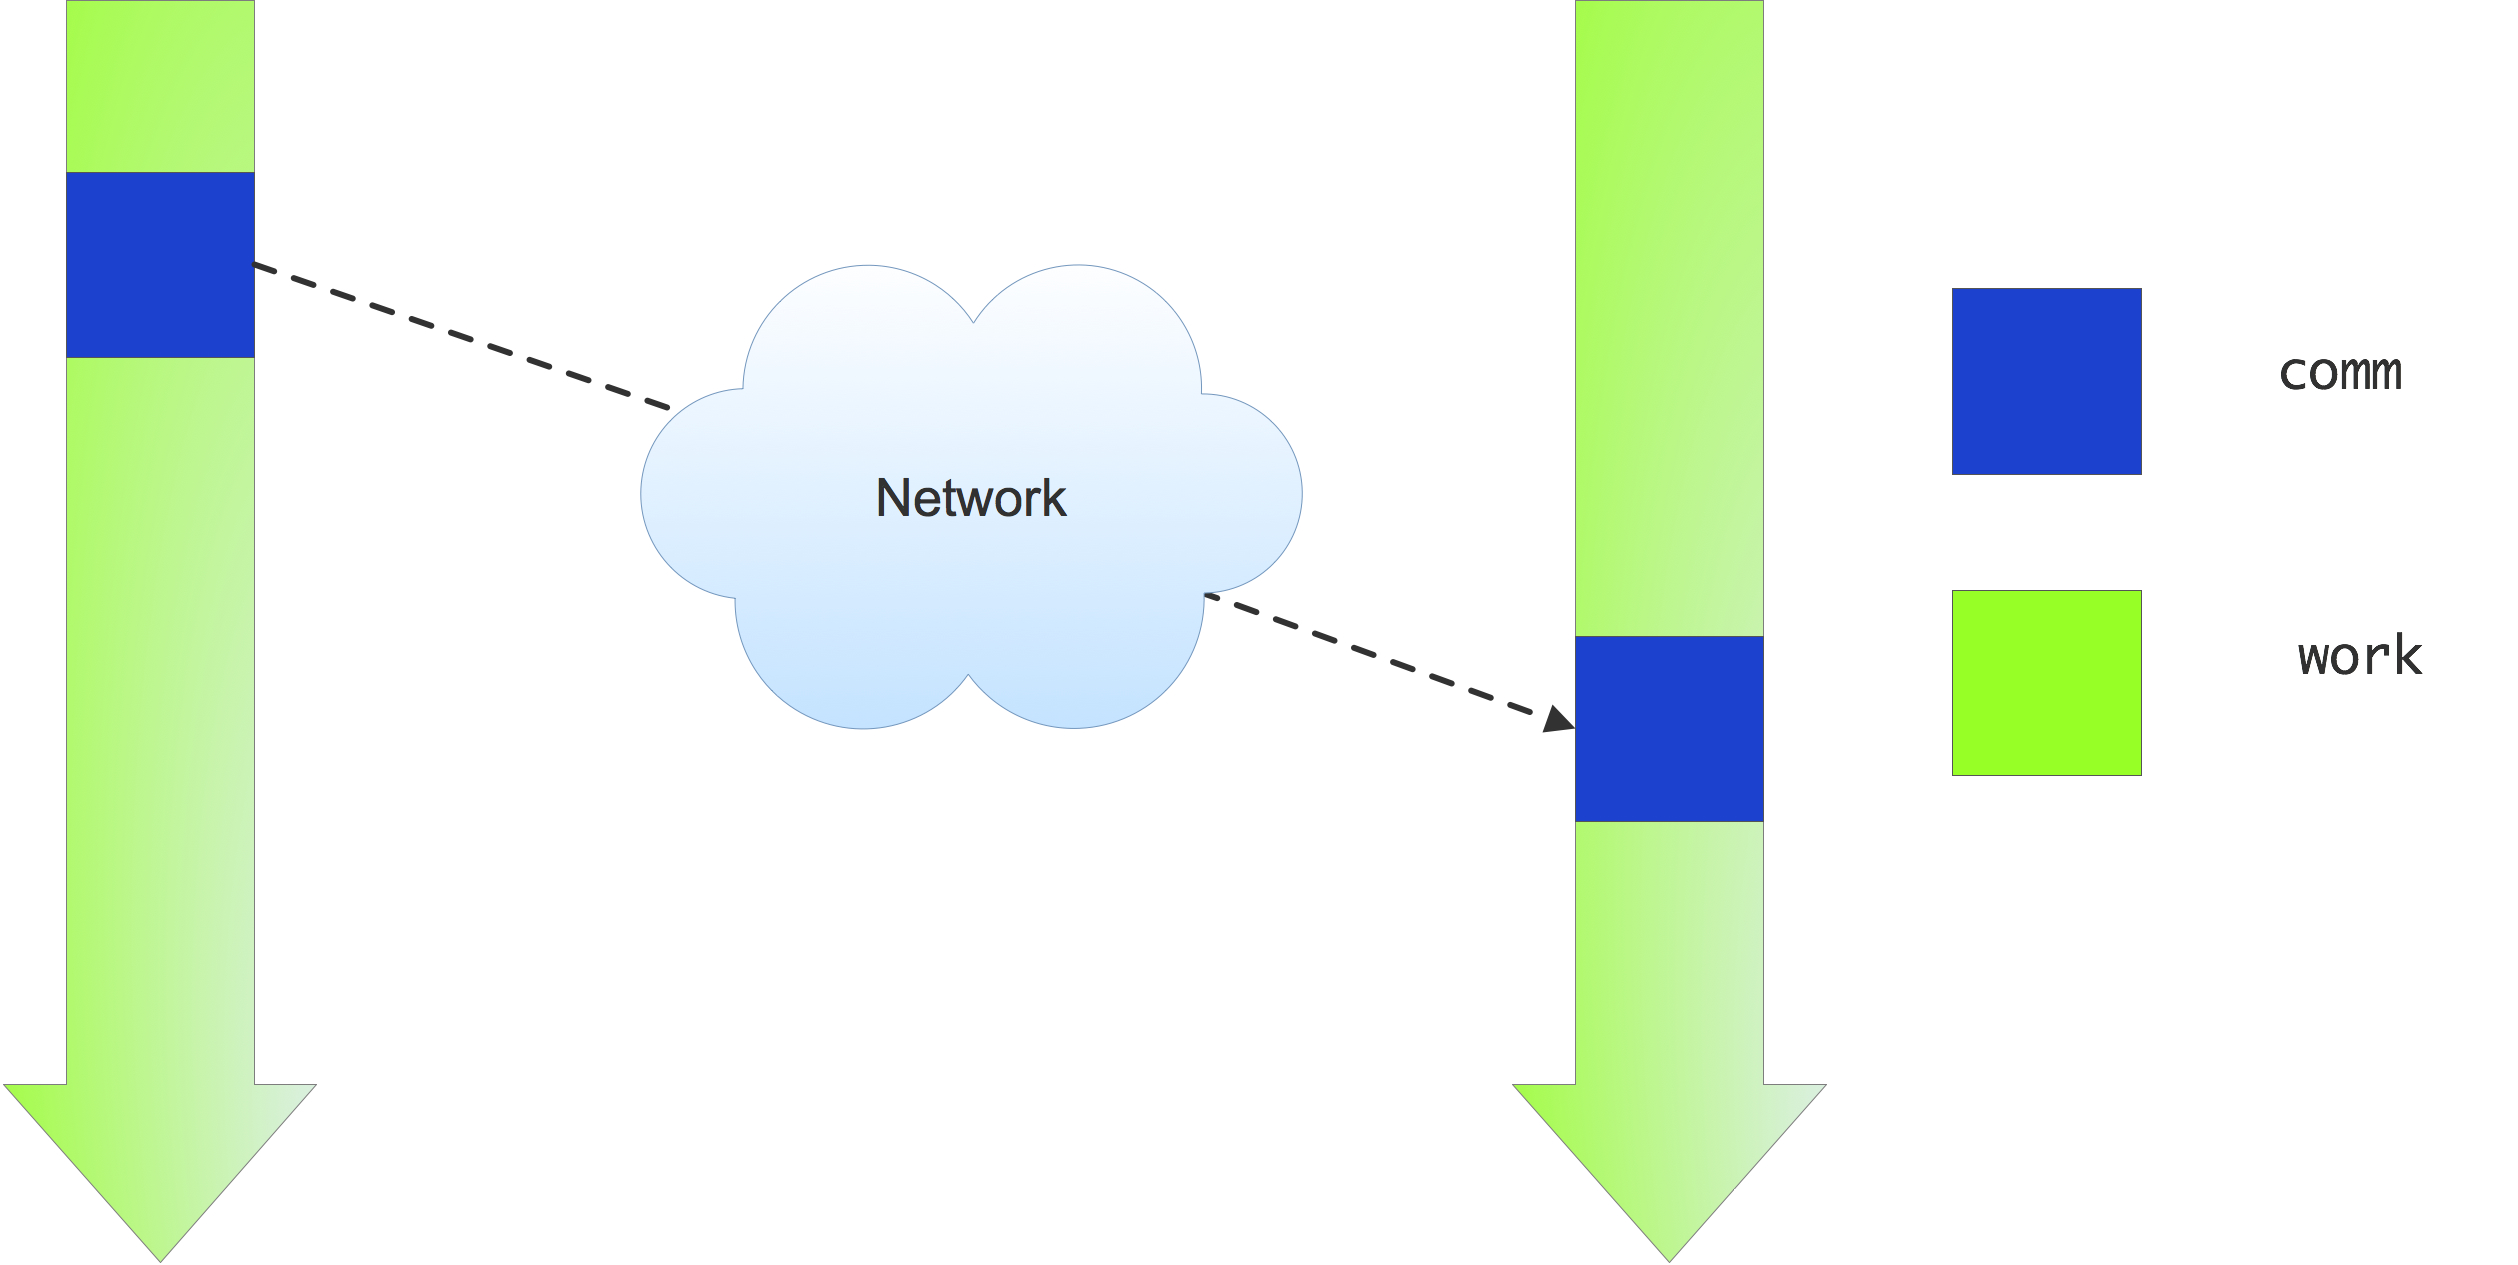
\includegraphics[scale=.08]{send-ideal}
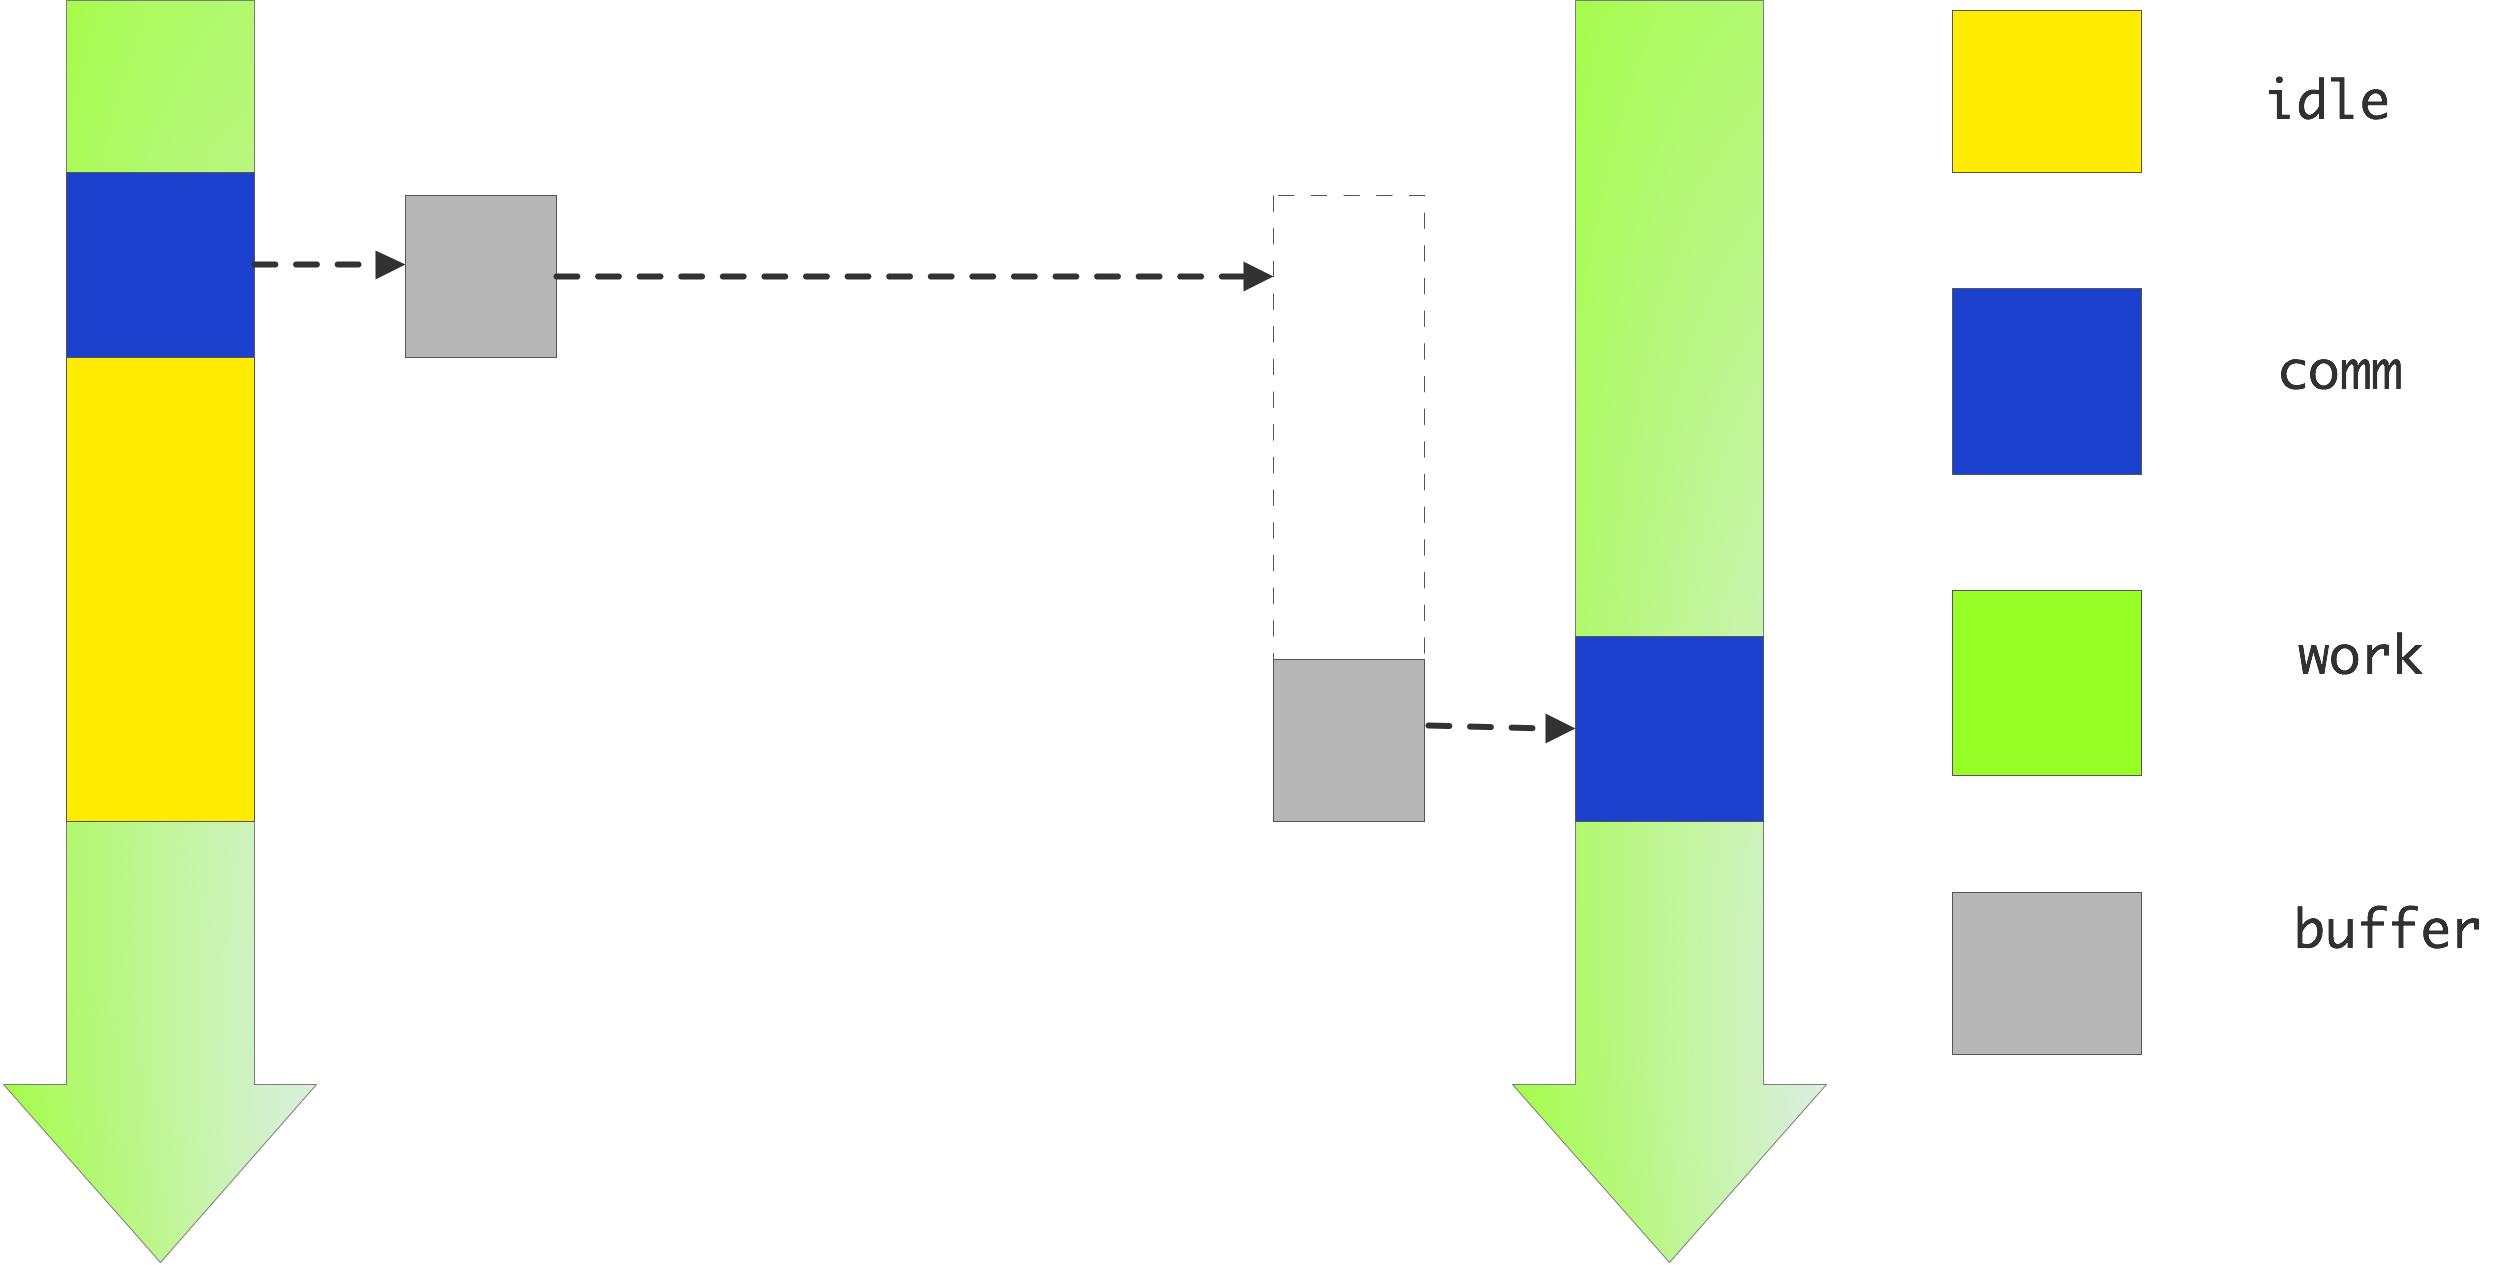
\includegraphics[scale=.08]{send-blocking}
\caption{Illustration of an ideal (left) and actual (right) send-receive interaction}
\label{fig:send-ideal}
\end{figure}
%
But this ideal scenario is not realistic: it assumes that somewhere
in the network there is buffer capacity for all messages that are in
transit.
This is not the case: data resides on the sender, and the sending call blocks,
until the receiver has received all of it. (There is a exception for
small messages, as explained in the next section.)

The use of \indexmpishow{MPI_Send} and \indexmpishow{MPI_Recv}
is known as \emph{blocking communication}: when your code reaches a
send or receive call, it blocks until the call is succesfully completed.
Technically, blocking operations are called
\emph{non-local}\index{operation!non-local} since their execution
depends on factors that are not local to the process.
See section~\ref{sec:mpi-local-non}.

\Level 2 {Deadlock}

Suppose two process need to exchange data, and consider the following
pseudo-code, which purports to exchange data between processes 0 and~1:
\begin{lstlisting}
other = 1-mytid; /* if I am 0, other is 1; and vice versa */
receive(source=other);
send(target=other);
\end{lstlisting}
Imagine that the two processes execute this code. They both issue the
send call\ldots\ and then can't go on, because they are both waiting
for the other to issue the send call corresponding to their receive call.
This is known as \indextermdef{deadlock}.

\Level 2 {Eager vs rendezvous protocol}
\label{sec:eager-limit}
\index{eager limit|(textbf}

Messages can be sent using (at least) two different
\indextermdef{protocol}s:
\begin{enumerate}
\item Rendezvous protocol, and
\item Eager protocol.
\end{enumerate}
The \indextermsub{rendezvous}{protocol} is the most general.
Sending a message takes several steps:
\begin{enumerate}
\item the sender sends a header,
  typically containing the \indextermbus{message}{envelope}:
  metadata describing the message;
\item the receiver returns a `ready-to-send' message;
\item the sender sends the actual data.
\end{enumerate}
The purpose of this is to to prepare the receiver buffer space
for large messages. However, it implies that the sender has to
wait for some return message from the receiver,
making the behavior a \indextermsub{synchronous}{message}.

For the eager protocol, consider the example:
\begin{lstlisting}
other = 1-mytid; /* if I am 0, other is 1; and vice versa */
send(target=other);
receive(source=other);
\end{lstlisting}
With a synchronous protocol you should get deadlock,
since the send calls will be waiting for the receive operation to be posted.

In practice, however, this code will often work. The reason is that
MPI implementations sometimes send small messages regardless of whether
the receive has been posted. This is known as an \indextermbus{eager}{send},
and it relies on the availability of
some amount of available buffer space. The size under which this behavior
is used is sometimes referred to as the \indextermbus{eager}{limit}.

\begin{comment}
  The following code is guaranteed to block, since a \indexmpishow{MPI_Recv}
  always blocks:
  \cverbatimsnippet[examples/mpi/c/recvblock.c]{recvblock}
  On the other hand, if we put the send call before the receive,
  code may not block for small messages
  that fall under the eager limit.
\end{comment}

To illustrate eager and blocking behavior in \indexmpishow{MPI_Send},
consider an example where we send
gradually larger messages. From the screen output you can see what
the largest message was that fell under the eager limit; after that the code
hangs because of a deadlock.
%
\cverbatimsnippet[examples/mpi/c/sendblock.c]{sendblock}
%
\fverbatimsnippet[examples/mpi/f/sendblock.F90]{sendblock-f}
%
\pverbatimsnippet[examples/mpi/p/sendblock.py]{sendblockp}

If you want a code to exhibit the same blocking behavior for  all message sizes,
you force the send call to be blocking by using
\indexmpishow{MPI_Ssend}, which has the same calling sequence as \indexmpishow{MPI_Send},
but which does not allow eager sends.
%
\cverbatimsnippet[examples/mpi/c/ssendblock.c]{ssendblock}
%
Formally you can describe deadlock as follows. Draw up a graph where
every process is a node, and draw a directed arc from process~A to~B if
A is waiting for~B. There is deadlock if this directed graph has a
loop.

The solution to the deadlock in the above example is to first do the
send from 0 to~1, and then from 1 to~0 (or the other way around). So
the code would look like:
\begin{lstlisting}
if ( /* I am processor 0 */ ) {
  send(target=other);
  receive(source=other);
} else {
  receive(source=other);
  send(target=other);
}
\end{lstlisting}

Eager sends also influences
\emph{non-blocking}\index{eager send!and non-blocking} sends.
The wait call after a non-blocking send
will return immediately, regardless any receive call,
if the message is under the eager limit:
%
\csnippetwithoutput{eagerisend}{code/mpi/c}{eageri}
%

The eager limit is implementation-specific.
For instance,
for \indextermbus{Intel}{MPI} there is a variable
\indextermtt{I_MPI_EAGER_THRESHOLD} (old versions) or \indextermtt{I_MPI_SHM_EAGER_THRESHOLD};
for \indexterm{mvapich2} it is \indextermtt{MV2_IBA_EAGER_THRESHOLD},
and for \indexterm{OpenMPI} the
\texttt{--mca} options \indextermtt{btl_openib_eager_limit} and
\indextermtt{btl_openib_rndv_eager_limit}.

\index{eager limit|)}

\Level 2 {Serialization}
\label{sec:serialization}

There is a second, even more subtle problem with blocking
communication. Consider the scenario where every processor needs to
pass data to its successor, that is, the processor with the next
higher rank. The basic idea would be to first send to your successor,
then receive from your predecessor. Since the last processor does not
have a successor it skips the send, and likewise the first processor
skips the receive. The pseudo-code looks like:
\begin{lstlisting}
successor = mytid+1; predecessor = mytid-1;
if ( /* I am not the last processor */ )
  send(target=successor);
if ( /* I am not the first processor */ )
  receive(source=predecessor)
\end{lstlisting}

\begin{exercise}
  \label{ex:serialsend}
  (Classroom exercise) Each student holds a piece of paper
  in the right hand --~keep your left hand behind your back~--
  and we want to execute:
  \begin{enumerate}
  \item Give the paper to your right neighbor;
  \item Accept the paper from your left neighbor.
  \end{enumerate}
  Including boundary conditions for first and last process, that becomes
  the following program:
  \begin{enumerate}
  \item If you are not the rightmost student, turn to the right
    and give the paper to your right neighbor.
  \item If you are not the leftmost student, turn to your left and
    accept the paper from your left neighbor.
  \end{enumerate}
\end{exercise}

This code does not deadlock. All processors but the last one block on
the send call, but the last processor executes the receive call. Thus,
the processor before the last one can do its send, and subsequently
continue to its receive, which enables another send, et cetera.

In one way this code does what you intended to do:
it will terminate (instead of hanging forever on a
deadlock) and exchange data the right way. However, the execution
now suffers from unexpected \indexterm{serialization}: only
one processor is active at any time, so what should have been a
%
\begin{figure}[ht]
\includegraphics[scale=.4]{linear-serial}
\caption{Trace of a simple send-recv code}
\label{fig:serialization}
\end{figure}
%
parallel operation becomes a sequential one. This is illustrated in
figure~\ref{fig:serialization}.

\begin{exercise}
  \label{ex:linear-sequential}
  Implement the above algorithm using \indexmpishow{MPI_Send} and \indexmpishow{MPI_Recv} calls.
  Run the code, and use TAU to reproduce the trace output 
  of figure~\ref{fig:serialization}.
  If you don't have TAU, can you show this serialization
  behavior using timings, for instance running it on an increasing number of processes?
  \skeleton{rightsend}
\end{exercise}

It is possible to orchestrate your processes to get an efficient and
deadlock-free execution, but doing so is a bit cumbersome.

\begin{exercise}
  The above solution treated every processor equally. Can you come up
  with a solution that uses blocking sends and receives, but does not
  suffer from the serialization behavior?
\end{exercise}

There are better solutions which we will
explore in the next section.

\Level 1 {Bucket brigade}
\label{sec:bucketbrigade}

The problem with the previous exercise was that an operation that was
conceptually parallel became serial in execution. On the other hand,
sometimes the operation is actually serial in nature. One example is
the \indextermdef{bucket brigade} operation, where a piece of data is
successively passed down a sequence of processors.

\begin{exercise}
  \label{ex:bucket-block}
  Take the code of exercise~\ref{ex:linear-sequential} and modify it
  so that the data from process zero gets propagated to every
  process. Specifically, compute all partial sums $\sum_{i=0}^pi^2$:
  \[ 
  \begin{cases}
    x_0 = 1&\hbox{on process zero}\\
    x_p = x_{p-1}+(p+1)^2 & \hbox{on process $p$}\\
  \end{cases}
  \]
  Use \indexmpishow{MPI_Send} and \indexmpishow{MPI_Recv}; make sure to get the order right.

  Food for thought: all quantities involved here are integers. Is it a good idea to
  use the integer datatype here?

  \skeleton{bucketblock}
\end{exercise}

\begin{remark}
  There is an \lstinline{MPI_Scan} routine (section~\ref{sec:scan})
  that performs the same computation,
  but computationally more efficiently. Thus, this exercise only serves to illustrate
  the principle.
\end{remark}

\index{communication!blocking|)}

\Level 1 {Pairwise exchange}
\label{sec:send-recv}

Above you saw that with blocking sends the precise ordering of the
send and receive calls is crucial. Use the wrong ordering and you get
either deadlock, or something that is not efficient at all in
parallel. MPI has a way out of this problem that is sufficient for
many purposes: the combined send/recv call \indexmpiref{MPI_Sendrecv}.

The sendrecv call works great if every process is paired
with precisely one sender and one receiver.
You would then write
\begin{lstlisting}
sendrecv( ....from... ...to... );
\end{lstlisting}
with the right choice of source and destination. For instance, to send
data to your right neighbor:
\begin{lstlisting}
MPI_Comm_rank(comm,&procno);
MPI_Sendrecv( .... 
    /* from: */ procno-1
     ... ... 
    /* to:   */ procno+1
     ... );
\end{lstlisting}
This scheme is correct for all processes but the first and last. 
In order to use the sendrecv call on these processes,
we use \indexmpishow{MPI_PROC_NULL} for the non-existing
processes that the endpoints communicate with.
\begin{lstlisting}
MPI_Comm_rank( .... &procno );
if ( /* I am not the first processor */ )
  predecessor = procno-1;
else
  predecessor = MPI_PROC_NULL;
if ( /* I am not the last processor */ )
  successor = procno+1;
else
  successor = MPI_PROC_NULL;
sendrecv(from=predecessor,to=successor);
\end{lstlisting}
where the sendrecv call is executed by all processors.

All processors but the last one send to their neighbor; the target
value of \indexmpishow{MPI_PROC_NULL} for
the last processor means a `send to the null processor': no actual
send is done. 

Likewise, receiving from \indexmpishow{MPI_PROC_NULL} succeeds without
altering the receive buffer.  The corresponding
\indexmpishow{MPI_Status} object has source
\indexmpishow{MPI_PROC_NULL}, tag \indexmpishow{MPI_ANY_TAG}, and
count zero.

\begin{remark}
  The \indexmpishow{MPI_Sendrecv} can inter-operate with
  the normal send and receive calls, both blocking and non-blocking.
  Thus it would also be possible to replace the \indexmpishow{MPI_Sendrecv}
  calls at the end points by simple sends or receives.
\end{remark}

\begin{mplnote}{Send-recv call}
  The send-recv call in \ac{MPL} has the same possibilities
  for specifying the send and receive buffer as the separate send and recv calls:
  scalar, layout, iterator. However, out of the nine conceivably possible
  routine signatures, only the versions are available where the send and receive buffer
  are specified the same way.
  Also, the send and receive tag need to be specified; they do not have default values.

  \cxxverbatimsnippet{mplsendrecv}% exercise, so no source
\end{mplnote}

\begin{exercise}
  \label{ex:rightsendrecv}
  Revisit exercise~\ref{ex:serialsend} and solve it using
  \indexmpishow{MPI_Sendrecv}.

  If you have TAU installed, make a trace. Does it look different
  from the serialized send/recv code? If you don't have TAU, run your
  code with different numbers of processes and show that the runtime
  is essentially constant.
  %\skeleton{rightsend}
\end{exercise}

This call makes it easy to exchange data between two processors: both
specify the other as both target and source. However, there need not
be any such relation between target and source: it is possible to
receive from a predecessor in some ordering, and send to a successor
in that ordering; see figure~\ref{fig:sendrecv}.

\begin{figure}[ht]
  \includegraphics[scale=.5]{sendrecv-right}
  \caption{An MPI Sendrecv call}
  \label{fig:sendrecv}
\end{figure}

\begin{figure}[ht]
  \includegraphics[scale=.4]{sendrecv-steps}
  \caption{Two steps of send/recv to do a three-point combination}
  \label{fig:sendrecv-steps}.
\end{figure}

For the above three-point combination scheme you need to move data
both left right, so you need two \indexmpishow{MPI_Sendrecv} calls;
see figure~\ref{fig:sendrecv-steps}.

\begin{exercise}
  \label{ex:3ptsendrecv}
  Implement the above three-point combination scheme using \indexmpishow{MPI_Sendrecv};
  every processor only has a single number to send to its neighbor.
  \skeleton{sendrecv}
\end{exercise}

Hints for this exercise:
\begin{itemize}
\item Each process does one send and one receive; if a process needs
  to skip one or the other, you can specify
  \indexmpidef{MPI_PROC_NULL} as the other process in the send or
  receive specification. In that case the corresponding action
  is not taken.
\item As with the simple send/recv calls, processes have to match up:
  if process~$p$ specifies $p'$ as the destination of the send part of
  the call, $p'$~needs to specify $p$ as the source of the recv part.
\end{itemize}

The following exercise lets you implement a sorting algorithm with the
send-receive call\footnote {There is an \n{MPI\_Compare\_and\_swap}
  call. Do not use that.}.

\begin{figure}[ht]
  \includegraphics[scale=.3]{swapsort1}
  \caption{Odd-even transposition sort on 4 elements.}
  \label{fig:swapsort1}
\end{figure}

\begin{exercise}
  \label{ex:exchangesort}
  A very simple sorting algorithm is \indextermsub{swap}{sort} or
  \indextermsub{odd-even transposition}{sort}:
  pairs of processors compare data, and if necessary exchange. The
  elementary step is called a \indexterm{compare-and-swap}: in a pair
  of processors each sends their data to the other; one keeps the
  minimum values, and the other the maximum.
  For simplicity, in this exercise we give each processor just a single number.

  The transposition sort algorithm is split in even and odd stages, where
  in the even stage processors $2i$ and $2i+1$ compare and swap data,
  and in the odd stage processors $2i+1$ and $2i+2$ compare and swap.
  You need to repeat this $P/2$ times, where $P$~is the number of
  processors; see figure~\ref{fig:swapsort1}.

  Implement this algorithm using \indexmpishow{MPI_Sendrecv}. (Use
  \indexmpishow{MPI_PROC_NULL} for the edge cases if needed.)
  Use a gather call to print the global state of the distributed array
  at the beginning and end of the sorting process.
\end{exercise}

\begin{figure}[ht]
  \includegraphics[scale=.3]{swapsort2}
  \caption{Odd-even transposition sort on 4 processes, holding 2 elements each.}
  \label{fig:swapsort2}
\end{figure}

\begin{remark}
  It is not possible to use \indexmpishow{MPI_IN_PLACE} for the buffers,
  as in section~\ref{sec:allreduce-inplace}.
  Instead, the routine \indexmpiref{MPI_Sendrecv_replace} has only one buffer,
  used as both send and receive buffer.
  Of course, this requires the send and receive messages
  to fit in that one buffer.
\end{remark}

\begin{exercise}
  Extend this exercise to the case where each process hold an equal
  number of elements, more than~1. Consider figure~\ref{fig:swapsort2}
  for inspiration. Is it coincidence that the algorithm takes the same
  number of steps as in the single scalar case?
\end{exercise}

\begin{mpifournote}{Non-blocking/persistent sendrecv}
  There are
  \emph{non-blocking}\index{non-blocking communication}
  and
  \emph{persistent}\index{persistent communication}
  versions of \indexmpishow{MPI_Sendrecv}:
  \indexmpidef{MPI_Isendrecv}, \indexmpidef{MPI_Sendrecv_init},
  \indexmpidef{MPI_Isendrecv_replace}, \indexmpidef{MPI_Sendrecv_replace_init}.
\end{mpifournote}
